% Beautified TikZ figure for tool overview
\newcommand{\iconinput}{%

\begin{tikzpicture}[x=1mm,y=1mm,baseline=-0.6ex]
\draw[line width=0.35pt,rounded corners=0.3pt] (0,0) -- (4,0) -- (4,4) -- (1.2,4) -- (0,2.8) -- cycle;
\draw[line width=0.3pt] (1.2,4) -- (1.2,2.8) -- (0,2.8);
\draw[line width=0.25pt] (0.8,1.0) -- (3.2,1.0);
\draw[line width=0.25pt] (0.8,1.8) -- (3.2,1.8);
\end{tikzpicture}%
}
\newcommand{\icontiler}{%

\begin{tikzpicture}[x=1mm,y=1mm,baseline=-0.6ex]
\draw[line width=0.35pt] (0,0) rectangle (4,4);
\draw[line width=0.25pt] (0,2) -- (4,2);
\draw[line width=0.25pt] (2,0) -- (2,4);
\fill[teal!35] (0,2) rectangle (2,4);
\fill[teal!15] (2,0) rectangle (4,2);
\end{tikzpicture}%
}
\newcommand{\iconcomb}{%
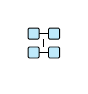
\begin{tikzpicture}[x=1mm,y=1mm,baseline=-0.6ex]
\draw[line width=0.3pt,rounded corners=0.4pt,fill=cyan!25] (0,2.5) rectangle (1.4,3.9);
\draw[line width=0.3pt,rounded corners=0.4pt,fill=cyan!25] (2.6,2.5) rectangle (4,3.9);
\draw[line width=0.3pt,rounded corners=0.4pt,fill=cyan!25] (0,0.1) rectangle (1.4,1.5);
\draw[line width=0.3pt,rounded corners=0.4pt,fill=cyan!25] (2.6,0.1) rectangle (4,1.5);
\draw[line width=0.25pt] (1.4,3.2) -- (2.6,3.2);
\draw[line width=0.25pt] (1.4,0.8) -- (2.6,0.8);
\draw[line width=0.25pt] (2,1.5) -- (2,2.5);
\end{tikzpicture}%
}
\newcommand{\iconexport}{%
\begin{tikzpicture}[x=1mm,y=1mm,baseline=-0.6ex]
\draw[line width=0.35pt,rounded corners=0.3pt] (0,0) rectangle (4,4);
\draw[line width=0.25pt] (0.7,3.0) -- (3.3,3.0);
\draw[line width=0.25pt] (0.7,2.2) -- (3.3,2.2);
\draw[line width=0.25pt] (0.7,1.4) -- (2.5,1.4);
\draw[-{Latex[length=1.3mm,width=0.9mm]},line width=0.28pt] (2.0,0.5) -- (3.5,0.5);
\end{tikzpicture}%
}
\newcommand{\iconviz}{%
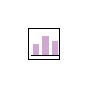
\begin{tikzpicture}[x=1mm,y=1mm,baseline=-0.6ex]
\draw[line width=0.3pt] (0,0) rectangle (4,4);
\fill[violet!35] (0.6,0.6) rectangle (1.4,2.0);
\fill[violet!35] (1.8,0.6) rectangle (2.6,3.0);
\fill[violet!35] (3.0,0.6) rectangle (3.8,2.4);
\draw[line width=0.25pt] (0.4,0.6) -- (3.9,0.6);
\end{tikzpicture}%
}
\newcommand{\icontest}{%

\begin{tikzpicture}[x=1mm,y=1mm,baseline=-0.6ex]
\draw[line width=0.3pt,rounded corners=0.4pt] (0,0) rectangle (4,4);
\draw[line width=0.4pt,green!60!black] (0.8,2.0) -- (1.8,1.1) -- (3.3,2.9);
\end{tikzpicture}%
}
\newcommand{\iconverilog}{%
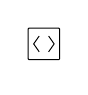
\begin{tikzpicture}[x=1mm,y=1mm,baseline=-0.6ex]
\draw[line width=0.35pt,rounded corners=0.3pt] (0,0) rectangle (4,4);
\draw[line width=0.35pt] (1.4,1.0) -- (0.7,2.0) -- (1.4,3.0);
\draw[line width=0.35pt] (2.6,1.0) -- (3.3,2.0) -- (2.6,3.0);
\end{tikzpicture}%
}
\newcommand{\iconhwsim}{%

\begin{tikzpicture}[x=1mm,y=1mm,baseline=-0.6ex]
\draw[line width=0.3pt,rounded corners=0.4pt] (0,0) rectangle (4,4);
\draw[line width=0.3pt] (0.4,1.0) -- (1.1,1.0) -- (1.1,3.0) -- (2.0,3.0) -- (2.0,1.4) -- (3.1,1.4) -- (3.1,2.6) -- (3.6,2.6);
\end{tikzpicture}%
}
\newcommand{\iconiropt}{%

\begin{tikzpicture}[x=1mm,y=1mm,baseline=-0.6ex]
\draw[line width=0.3pt,rounded corners=0.4pt] (0,0) rectangle (4,4);
\draw[line width=0.45pt,fill=yellow!50,draw=orange!80!black]
  (2.5,3.7) -- (1.2,2.2) -- (2.0,2.2) -- (1.5,0.3) -- (2.8,1.8) -- (2.0,1.8) -- cycle;
\end{tikzpicture}%
}

\begin{tikzpicture}[
    node distance=1.0cm and 0.75cm,
    font=\sffamily,
    stage/.style={
        rectangle,
        rounded corners=3pt,
        draw=black!70,
        line width=0.9pt,
        minimum width=2.15cm,
        minimum height=1.35cm,
        align=center,
        font=\large,
        text=black
    },
    stagewide/.style={
        stage,
        minimum width=2.45cm
    },
    artifact/.style={
        rectangle,
        rounded corners=2pt,
        draw=black!55,
        line width=0.8pt,
        fill=white,
        minimum width=1.25cm,
        minimum height=0.72cm,
        align=center,
        font=\Large
    },
    result/.style={
        circle,
        draw=black!65,
        line width=0.85pt,
        minimum size=0.95cm,
        align=center,
        font=\Large
    },
    link/.style={-{Latex[length=3.0mm,width=2.0mm]}, line width=0.95pt, draw=black!75}
]

% Main left-to-right pipeline
\node[stage, fill=blue!18] (input) {\iconinput\\Input Specs\\(Base, Size)};
\node[stage, fill=teal!18, right=of input] (tiler) {\icontiler\\Tiler};
\node[stagewide, fill=cyan!18, right=of tiler] (combgen) {\iconcomb\\Decomposition\\Combinations};

% Parallel branch after decomposition
\node[stagewide, fill=orange!24, right=of combgen, xshift=0.25cm, yshift=0.95cm] (exporter) {\iconexport\\IR\\Generator};
\node[stagewide, fill=yellow!22, right=of exporter] (iropt) {\iconiropt\\IR\\Optimizer};
\node[stage, fill=violet!20, right=of combgen, xshift=0.25cm, yshift=-0.95cm] (visualizer) {\iconviz\\Visualizer};

% Visualizer output tile map icon
\node[
    draw,
    rounded corners=2pt,
    line width=0.8pt,
    inner sep=2pt,
    minimum width=1.3cm,
    minimum height=1.3cm,
    right=of visualizer,
    xshift=0.15cm,
    fill=white
] (pdfout) {
    \begin{tikzpicture}[scale=0.44]
        \draw[line width=0.35pt, draw=black!60] (0,0) grid[step=0.5] (2,2);
        \fill[blue!35]   (0,1)   rectangle (0.5,1.5);
        \fill[teal!35]   (0.5,1) rectangle (1,1.5);
        \fill[red!35]    (1,1)   rectangle (1.5,1.5);
        \fill[yellow!45] (1.5,1) rectangle (2,1.5);
    \end{tikzpicture}
};

% Software and hardware flow on the right
\node[stagewide, fill=red!22, right=of iropt, xshift=0.7cm, yshift=0.95cm] (tester) {\icontest\\Software\\Simulation};
\node[stage, fill=green!22, right=of iropt, xshift=0.7cm, yshift=-1.1cm] (verilog) {\iconverilog\\RTL\\Generator};
\node[stagewide, fill=lime!22, right=of verilog, xshift=0.15cm] (hwsim) {\iconhwsim\\Hardware\\Simulation};

% Output artifacts
\node[artifact, below=0.6cm of verilog, xshift=-1.3cm] (file1) {.v};
\node[artifact, below=0.6cm of verilog] (file2) {.tcl};
\node[artifact, below=0.6cm of verilog, xshift=1.3cm] (file3) {.xdc};

% Result badges
\coordinate (testcenter) at (hwsim.center |- tester.center);
\node[result, fill=green!35, at={($(testcenter)+(-0.62cm,0)$)}] (testpass) {\checkmark};
\node[result, fill=red!35, at={($(testcenter)+(0.62cm,0)$)}] (testfail) {$\times$};
\node[draw, rounded corners=2pt, line width=0.8pt, fit={(testpass) (testfail)}, inner sep=0.2cm] (testbox) {};

% Routing
\draw[link] (input) -- (tiler);
\draw[link] (tiler) -- (combgen);

\draw[line width=0.95pt, draw=black!70] (combgen.east) -- ++(0.58,0) coordinate (split1);
\draw[link] (split1) |- (exporter.west);
\draw[link] (split1) |- (visualizer.west);
\draw[link] (visualizer.east) -- (pdfout.west);

\draw[link] (exporter) -- (iropt);
\draw[link] (exporter.north) -- ++(0,1.5) -| (tester.north);
\draw[line width=0.95pt, draw=black!70] (iropt.east) -- ++(0.5,0) coordinate (split2);
\draw[link] (split2) |- (tester.west);
\draw[link] (split2) |- (verilog.west);

\draw[link] (tester.east) -- (testbox.west);
\draw[link] (verilog) -- (hwsim);
\draw[link] (hwsim) -- (testbox);

\draw[link] (verilog) -- (file1);
\draw[link] (verilog) -- (file2);
\draw[link] (verilog) -- (file3);

\end{tikzpicture}
